\chapter{Creating a test suite: the "tests" folder}
\label{chap:creating_a_test_suite}

\section{Methodology}

Writing a Parsing Expression Grammar (see next part of the thesis) requires constant vigilance in order to make sure
that any rule change doesn't impact several nodes of the grammar at the same time, thus breaking its parse tree. Running test
sentences one by one, by hand, would be time consuming and not very scientific (especially if there are hundreds of test sentences).\newline

In order to evaluate scientifically the validity and degree of completeness of the code and grammar produced, a test suite must be created.
Additionally, a data set with enough sentences to evaluate is required. Thankfully, throughout the chapters of \citetitle{cowan1997complete},
\citeauthor{cowan1997complete} gives us a trove of example sentences.\newline

Using the PyTest Python library \footcite{pytest8.3.2}, a test suite will be constructed in order to run the "grammar\_parser" module
and the "visitor" module on all sentences collected.

\section{Breakdown of the folder}

The code produced is found at Annex \ref{appendix:parser-testing-annex}. You may read it along the following explanations.

\newpage

\subsection*{conftest.py file}

This file has two functions: \newline

The \textbf{sentences} function lists all files present in the "sentences" folder and opens them one by one,
in order to collect the test sentences. For each sentence, we also list what chapter it comes from (through the file name) and
at what line in the test file it located at.\newline

The \textbf{build\_test\_parameters} function uses the previous function as a PyTest fixture, in order to yield the test sentences and
their context one by one to the actual test function, found in the next file.

\subsection*{test\_gentufa\_and\_visitor.py file}

In this file, outside of the test function, an instance of the Gentufa class is created, which will be used to parse all test sentences.\newline

The test function, called \textbf{test\_chapter\_sentences}, receives the sentences one by one thanks to the \textbf{build\_test\_parameters} function
described above. For each sentence, we first run the parser, marking the test as a failure if the parser returns an exception (either IncompleteParseError
or ParseError). Then, the parse tree generated is fed to an instance of the GentufaVisitor class, and we check if the "visit" worked fine and if the output
has a valid format. If an exception was raised (either VisitationError or TypeError), we mark the test as a failure.

\subsection*{sentences directory}

The "sentences" directory contains many files, one per chapter, listing all the sentences which will compose the dataset.
All test sentences are surrounded by comments giving context about which chapter and section of the book they come from.

\newpage

\begin{lstlisting}[caption=Example of a test file with some sentences to be parsed]
### Chapter 2.5 ###
# Example 2.11
mi tavla do zo'e zo'e
# Example 2.12
do tavla mi ta zo'e
# Example 2.13
mi tavla zo'e tu ti
# Example 2.14
mi tavla do
# Example 2.15
do tavla mi ta
\end{lstlisting}

\newpage

\section{Examples of usage}

The test suite is run by executing a makefile at the root of the code directory with the following command: \textbf{make tests}.
Once executed, all tests will run and a test run summary is displayed. There are two possible outcomes: either all tests pass correctly,
or errors have been introduced. \newline

Thankfully, due to proper error-handling and test cases management, the test suite outputs for each error:

\begin{itemize}
    \item what sentence the error corresponds to, which file it comes from, and at which line it is in the file (which is useful due to the
    added context given in the test files which was explained previously)
    \item whether it was the Parser class that failed, or the Visitor class
    \item above the test run summary each error is displayed with a traceback, which thanks to Parsimonious' \footcite{parsimonious} good error
    handling highlights explicitly which part of the grammar or the visitor is failing.
\end{itemize}

This is extremely useful in order to debug at which layer the error was introduced. \newline

The following figures display examples of these two possible outcomes:\newline

\begin{figure}[H]
\hspace{-1.1cm}
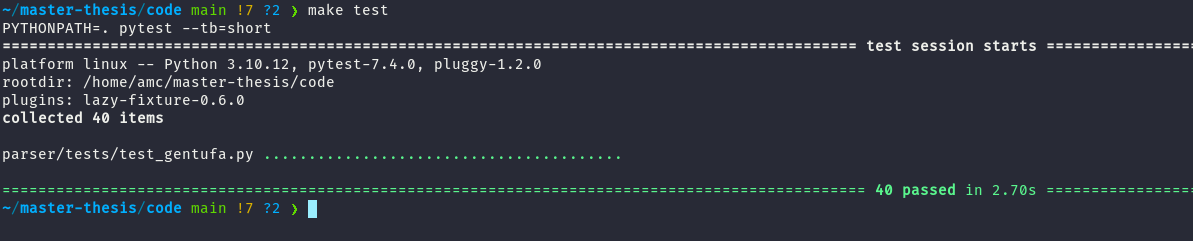
\includegraphics[scale=0.43]{images/pytest_output_pass.png}
\caption{Pytest Output Example - All tests passing}
\end{figure}

\begin{figure}[H]
\hspace{-1.8cm}
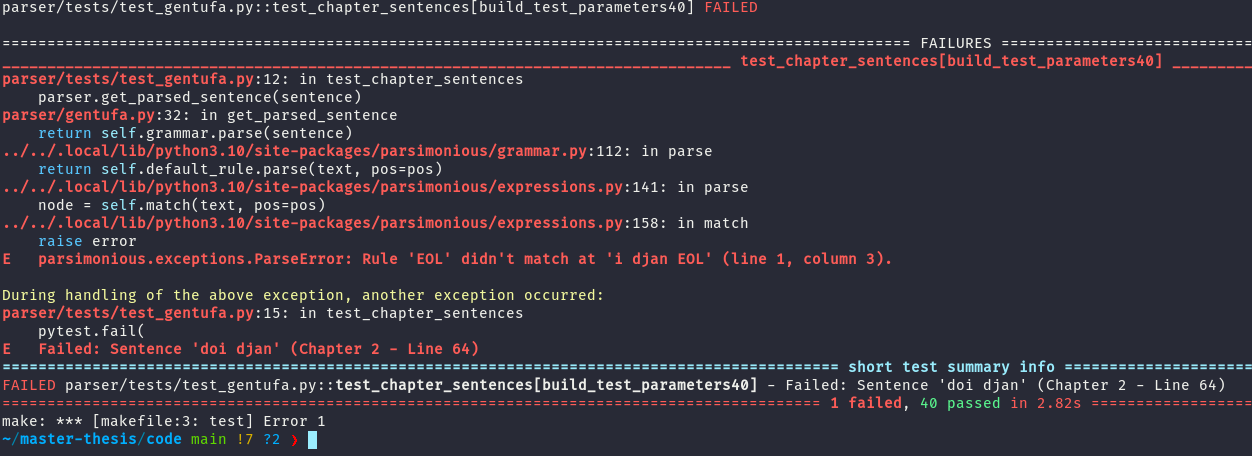
\includegraphics[scale=0.30]{images/pytest_output_fail.png}
\caption{Pytest Output Example - An error occured}
\end{figure}